\chapter{Requirement Specifications} \label{chap:reqs} \label{chap:requirements}

\section{Existing System}
Existing recruitment mechanisms and job aggregator platforms in the local and global context focus primarily on passive job posting and uncoordinated resume aggregation. Job postings are often published with minimal structural criteria, resumes are submitted as static documents into crowded email inboxes or unparsed databases, and candidate evaluation is handled manually or through primitive keyword-matching scripts \cite{parasuraman2021ats}. In conventional workflows, recruiters spend an average of only six seconds manually scanning each resume, leading to subjective evaluation biases, human cognitive fatigue, and high turnaround times. When first-generation legacy Applicant Tracking Systems (ATS) are deployed, they rely on rigid substring matching that rejects qualified applicants who omit exact keyword synonyms, while rewarding candidates who artificially ``stuff'' keywords into their CVs \cite{roy2020resume}. Furthermore, applicants face a total ``black hole'', receiving no diagnostic feedback regarding why their application was disqualified or what skills were missing.

Key limitations of existing systems include:
\begin{itemize}
    \item \textbf{Cognitive Fatigue and High Time-to-Hire:} Manual screening of hundreds of unstructured resumes causes severe operational bottlenecks and inconsistent candidate assessments.
    \item \textbf{Syntactic Rigidity and False Disqualifications:} Legacy keyword filters fail to recognize contextual synonyms, domain hierarchies, or transferrable technical competencies.
    \item \textbf{Vulnerability to Keyword Stuffing:} Naive keyword frequency parsers are easily manipulated by unqualified candidates who pack job description text into their resumes.
    \item \textbf{Complete Candidate Feedback Void:} Job seekers receive no transparency into their computed ATS compatibility scores or missing skill gaps.
    \item \textbf{Unverified Employer Postings:} Open job boards allow unverified accounts to post fraudulent listings, putting candidate personal data at risk.
    \item \textbf{Disjointed Pipeline Tracking:} Employers rely on separate offline spreadsheets to track candidate hiring stages due to lack of integrated stage management.
\end{itemize}

\section{Proposed System}
\textbf{RecruitSense} is proposed as an intelligent, multi-channel recruitment ecosystem, Applicant Tracking System (ATS), and Candidate Intelligence Platform engineered to streamline recruitment workflows, automate candidate screening, deliver explainable feedback, and provide recruiters with conversational resume deep-dives. The platform is architected as a decoupled, multi-tier microservices ecosystem consisting of:
\begin{enumerate}
    \item A responsive Single Page Application (SPA) frontend built with React 18, Vite, and Tailwind CSS.
    \item A cross-platform mobile application engineered with Flutter and Dart for Android and iOS.
    \item A high-throughput RESTful API gateway engineered with Laravel 11 and MySQL 8.0.
    \item An asynchronous AI inference microservice developed with Python FastAPI, ChromaDB, and local LLaMA 3.2.
    \item A Retrieval-Augmented Generation (RAG) candidate intelligence engine powered by the ChromaDB vector database and dense sentence transformer embeddings (\texttt{all-MiniLM-L6-v2} / \texttt{nomic-embed-text}) \cite{lewis2020rag, malkov2018hnsw}.
\end{enumerate}

Major capabilities of the proposed system include:
\begin{itemize}
    \item \textbf{Automated AI-Powered Resume Screening:} Converts unstructured PDF resumes into normalized text streams, extracts candidate competencies, and computes a multi-attribute ATS match score ($0\% - 100\%$) against job descriptions.
    \item \textbf{Candidate Retrieval-Augmented Generation (RAG) Chat:} Enables recruiters to ask natural-language questions about candidates, retrieving semantically relevant text chunks from resumes with source citation evidence.
    \item \textbf{Skill Gap Diagnostics and Automated Course Pathways:} Automatically categorizes competencies into matched, missing, and bonus skills, and provides rejected candidates with targeted online course recommendations to upskill.
    \item \textbf{Dynamic AI Assessment Quiz Generation:} Automatically generates technical multiple-choice quizzes tailored to required job skills for candidate pre-screening.
    \item \textbf{Multi-Channel Role-Based Workspaces:} Delivers synchronized, role-based dashboards on Web and Mobile for Job Seekers (profile, experience tracking, job alerts, recommended jobs, application tracking) and Corporate Recruiters (candidate discovery, Kanban pipeline, analytics, interview scheduling).
    \item \textbf{Live Community Feed and Professional Networking:} Provides interactive social networking feeds for job seekers and employers to share professional updates, insights, and industry discussions.
    \item \textbf{Corporate Email Domain Verification:} Protects job seekers by enforcing custom domain validation rules (\texttt{TrustedEmailDomain}) to prevent fraudulent employer registrations.
    \item \textbf{Structured Hiring Pipeline Management:} Enables recruiters to manage candidate lifecycles across dynamic stages (\textit{Applied} $\rightarrow$ \textit{Screening} $\rightarrow$ \textit{Shortlisted} $\rightarrow$ \textit{Interview} $\rightarrow$ \textit{Offer/Rejected}).
\end{itemize}

\section{Requirement Specifications}

\subsection{Functional Requirements}
Functional requirements define the specific behaviors, operations, and services that RecruitSense must provide to its users. They are derived directly from system use cases and stakeholder goals. Table \ref{tab:functional_reqs} enumerates all functional requirements with their unique identifiers and descriptions.

\begin{table}[H]
\centering
\small
\caption{Functional Requirements for RecruitSense}
\label{tab:functional_reqs}
\begin{tabular}{|l|p{12cm}|}
\hline
\textbf{ID} & \textbf{Functional Requirement Description} \\ \hline
\textbf{FR-01} & \textbf{User Registration and Authentication:} Allow users to register as Job Seekers, Recruiters, or Admins and authenticate securely via Laravel Sanctum bearer tokens and Google OAuth. \\ \hline
\textbf{FR-02} & \textbf{Profile and Experience Management:} Enable Job Seekers and Employers to maintain profiles, experience records, bios, and account settings. \\ \hline
\textbf{FR-03} & \textbf{Corporate Domain Verification:} Validate recruiter registration emails against corporate domain whitelists, blocking public disposable email providers. \\ \hline
\textbf{FR-04} & \textbf{Create and Publish Job Vacancies:} Allow recruiters to create job postings with structured criteria (title, department, salary, description, required skills, experience). \\ \hline
\textbf{FR-05} & \textbf{Search and Multi-Filter Job Listings:} Provide job seekers with real-time job searching and multi-parameter filtering (keywords, location, employment type, salary). \\ \hline
\textbf{FR-06} & \textbf{Submit Job Application:} Enable job seekers to apply to vacancies by uploading their resume in PDF format with optional cover notes. \\ \hline
\textbf{FR-07} & \textbf{AI PDF Text Extraction:} Ingest uploaded resume documents and extract sanitized UTF-8 text streams page-by-page using the FastAPI AI microservice. \\ \hline
\textbf{FR-08} & \textbf{Skill Extraction and Boundary Matching:} Extract candidate skills using boundary-delimited regular expressions against a curated multi-domain technology taxonomy. \\ \hline
\textbf{FR-09} & \textbf{Dense Semantic Vector Embedding:} Generate high-dimensional vector embeddings and index resume context chunks into ChromaDB. \\ \hline
\textbf{FR-10} & \textbf{Composite Semantic ATS Score Formulation:} Compute a weighted ATS match percentage ($0\% - 100\%$) combining skill fulfillment and semantic vector similarity. \\ \hline
\textbf{FR-11} & \textbf{Skill Gap Diagnostics Visualization:} Display color-coded badges for matched skills, missing skills, and bonus skills to candidates and recruiters. \\ \hline
\textbf{FR-12} & \textbf{AI-Ranked Applicant Shortlist:} Display candidate applications to recruiters sorted in descending order of calculated ATS score. \\ \hline
\textbf{FR-13} & \textbf{Hiring Pipeline Stage Management:} Allow recruiters to transition candidate statuses across stages (\textit{Applied}, \textit{Screening}, \textit{Shortlisted}, \textit{Interview}, \textit{Offer}, \textit{Rejected}). \\ \hline
\textbf{FR-14} & \textbf{Interview Scheduling:} Enable recruiters to configure interview dates, times, and physical or virtual meeting locations for shortlisted candidates. \\ \hline
\textbf{FR-15} & \textbf{Save and Bookmark Jobs:} Allow job seekers to bookmark jobs of interest into a personal saved jobs list for future review. \\ \hline
\textbf{FR-16} & \textbf{Real-Time In-App Messaging:} Enable direct messaging between job seekers and recruiters to coordinate application details. \\ \hline
\textbf{FR-17} & \textbf{Notification System:} Dispatch real-time in-app alerts for application status changes, new messages, and scheduled interviews. \\ \hline
\textbf{FR-18} & \textbf{Report Fraudulent Postings:} Allow job seekers to report suspicious or misleading job listings for administrative investigation. \\ \hline
\textbf{FR-19} & \textbf{Admin Moderation Console:} Provide administrators with tools to moderate employers, review flagged listings, and suspend abusive user accounts. \\ \hline
\textbf{FR-20} & \textbf{Platform Analytics Dashboard:} Provide administrators and recruiters with statistical dashboards showing applicant distributions and match metrics. \\ \hline
\textbf{FR-21} & \textbf{Candidate RAG Conversational Chat:} Enable recruiters to query candidate qualifications through semantic dense vector search and grounded context generation using ChromaDB. \\ \hline
\textbf{FR-22} & \textbf{Cross-Platform Flutter Mobile Workspaces:} Deliver synchronized native mobile applications for Android and iOS providing candidate discovery, job alerts, and pipeline tracking. \\ \hline
\textbf{FR-23} & \textbf{Automated Skill Gap Course Recommendations:} Recommend curated online courses (Coursera, edX, Udemy) tailored to candidate missing competencies. \\ \hline
\textbf{FR-24} & \textbf{Automated AI Assessment Quiz Generation:} Dynamically generate multiple-choice skill assessment tests based on required vacancy competencies. \\ \hline
\textbf{FR-25} & \textbf{Community Feed and Professional Networking:} Provide a community discussion wall where users share professional posts, comments, and connection networks. \\ \hline
\end{tabular}
\end{table}

\subsection{Non-Functional Requirements}
Non-functional requirements specify quality constraints, security parameters, and operational attributes governing the system architecture. Table \ref{tab:non_functional_reqs} summarizes the key non-functional requirements.

\begin{table}[H]
\centering
\small
\caption{Non-Functional Requirements for RecruitSense}
\label{tab:non_functional_reqs}
\begin{tabular}{|l|p{12cm}|}
\hline
\textbf{ID} & \textbf{Non-Functional Requirement Description} \\ \hline
\textbf{NFR-01} & \textbf{Performance and Latency:} Ensure standard REST API responses occur within $300\text{ ms}$, RAG semantic queries respond in under $1.5\text{ seconds}$, and ATS scoring executes under $2.0\text{ seconds}$. \\ \hline
\textbf{NFR-02} & \textbf{Authentication and Token Security:} Protect all authenticated API endpoints with Laravel Sanctum bearer tokens hashed with SHA-256 in database storage. \\ \hline
\textbf{NFR-03} & \textbf{Data Protection and Hashing:} Hash all user passwords using Bcrypt with a minimum work factor of 12 rounds to protect against brute-force attacks. \\ \hline
\textbf{NFR-04} & \textbf{Input Sanitization and SQLi Prevention:} Neutralize SQL injection vulnerabilities by executing all queries through Eloquent ORM parameterized statements. \\ \hline
\textbf{NFR-05} & \textbf{Multi-Platform Responsiveness and UI Fluidity:} Provide an intuitive web interface with Tailwind CSS and a mobile application running at consistent 60 frames-per-second. \\ \hline
\textbf{NFR-06} & \textbf{System Reliability and Fault Tolerance:} Gracefully handle AI microservice timeouts and document extraction errors without corrupting core database state. \\ \hline
\textbf{NFR-07} & \textbf{Horizontal Scalability and Async I/O:} Implement asynchronous non-blocking request processing via FastAPI and ChromaDB vector indexing. \\ \hline
\textbf{NFR-08} & \textbf{Secure File Storage:} Validate uploaded file MIME types, enforce a 5MB size limit, and obfuscate file names with randomized UUID hashes outside public web roots. \\ \hline
\textbf{NFR-09} & \textbf{Maintainability and Modular Architecture:} Adhere to standard MVC in Laravel, Provider pattern in Flutter, and service-oriented design in FastAPI. \\ \hline
\textbf{NFR-10} & \textbf{CORS and Transport Encryption:} Enforce HTTPS across all network channels and configure strict Cross-Origin Resource Sharing (CORS) whitelists. \\ \hline
\end{tabular}
\end{table}

\section{System Use Case Modeling}
Use case modeling provides a high-level visual representation of how system actors interact with RecruitSense. The system identifies four primary actors:
\begin{enumerate}
    \item \textbf{Guest / Unregistered Visitor:} Can browse public job listings and initiate registration.
    \item \textbf{Job Seeker (Candidate):} Can manage profiles, search and filter jobs, submit resumes, view ATS match scores and skill gap feedback, track application pipelines, and message recruiters.
    \item \textbf{Corporate Recruiter / Employer:} Can create company profiles, publish job postings with skill requirements, review AI-ranked candidate shortlists, update hiring pipeline stages, schedule interviews, and message candidates.
    \item \textbf{System Administrator:} Can oversee user management, verify corporate domains, moderate flagged content, and inspect platform analytics.
    \item \textbf{AI Screening Engine (System Actor):} Autonomously parses uploaded PDF documents, extracts domain skills, indexes dense vectors into ChromaDB, and calculates semantic ATS match scores.
\end{enumerate}

Figure \ref{fig:overall_usecase} illustrates the comprehensive system use case model for RecruitSense.

\begin{figure}[H]
\centering
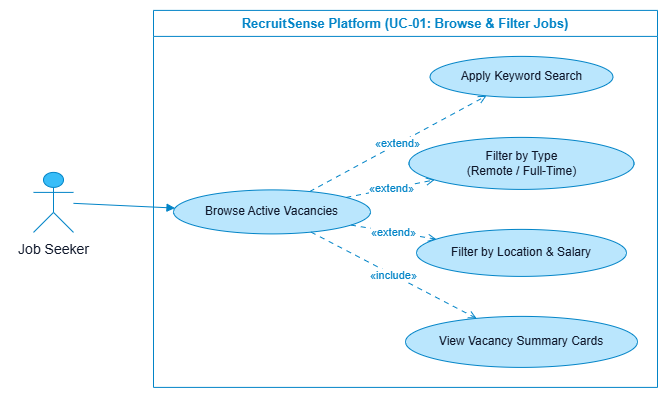
\includegraphics[width=0.85\linewidth]{figures/usecase_model.png}
\caption{System Use Case Model for RecruitSense}
\label{fig:overall_usecase}
\end{figure}

\section{Detailed Use Cases}

\subsection{Browse and Filter Jobs (UC-01)}
When a user accesses the RecruitSense web portal or mobile application, they can immediately explore active job listings published by verified corporate employers. The browsing interface provides an intuitive search bar allowing users to query job titles, technology stacks, or keywords. Users can refine search results using dynamic multi-attribute filters such as employment type (Full-time, Part-time, Remote, Contract), minimum salary threshold, department category, and geographic location. Each listing card presents key metadata including company name, location, salary badge, and required technical skills. Selecting a listing opens a comprehensive view detailing role responsibilities, required qualifications, and an instant application trigger. Unauthenticated guests can freely browse listings, while bookmarking vacancies and submitting applications require an authenticated Job Seeker account. This workflow is depicted in Figure \ref{fig:uc01_diag} and summarised in Table \ref{tab:uc01_spec}.

\begin{figure}[H]
\centering
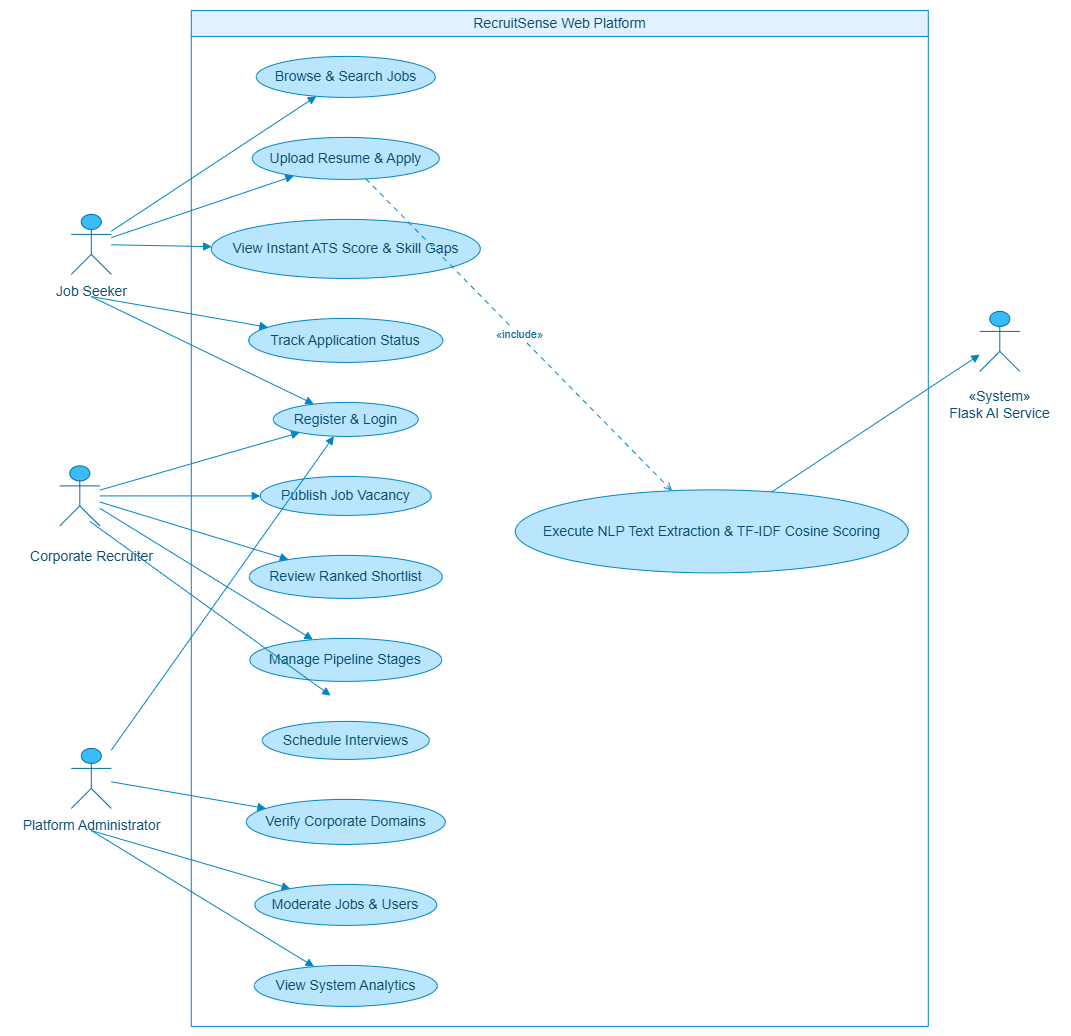
\includegraphics[width=0.65\linewidth]{figures/usecase_browse.png}
\caption{Browse and Filter Jobs Use Case Diagram}
\label{fig:uc01_diag}
\end{figure}

\begin{table}[H]
\centering
\small
\caption{Use Case: Browse and Filter Jobs (UC-01)}
\label{tab:uc01_spec}
\begin{tabular}{|p{3.2cm}|p{5.5cm}|p{5.5cm}|}
\hline
\textbf{Use Case ID:} & \multicolumn{2}{p{11.4cm}|}{UC-01} \\ \hline
\textbf{Use Case Name:} & \multicolumn{2}{p{11.4cm}|}{Browse and Filter Jobs} \\ \hline
\textbf{Created By:} & \multicolumn{2}{p{11.4cm}|}{Hamza Zahoor} \\ \hline
\textbf{Last Updated By:} & \multicolumn{2}{p{11.4cm}|}{Haseeb Ahmed} \\ \hline
\textbf{Actors:} & \multicolumn{2}{p{11.4cm}|}{Guest, Registered Job Seeker} \\ \hline
\textbf{Description:} & \multicolumn{2}{p{11.4cm}|}{User searches, filters, and views published job openings on the web and mobile portals.} \\ \hline
\textbf{Trigger:} & \multicolumn{2}{p{11.4cm}|}{User navigates to the platform job exploration portal.} \\ \hline
\textbf{Preconditions:} & \multicolumn{2}{p{11.4cm}|}{Platform web/mobile services and database are operational. \newline At least one active job vacancy exists in the system.} \\ \hline
\textbf{Post conditions:} & \multicolumn{2}{p{11.4cm}|}{Matching job vacancy cards and detailed job modals are rendered to the user.} \\ \hline
\multirow{4}{*}{\textbf{Normal Flow:}} & \multicolumn{1}{c|}{\textbf{Actor}} & \multicolumn{1}{c|}{\textbf{System}} \\ \cline{2-3}
& 1. User enters search keywords or selects a job category. & 2. System queries database and retrieves matching active listings. \vspace{2pt} \\
& 3. User selects filter criteria (Remote, Full-time, Salary). & 4. System dynamically updates the list view without full page reload. \vspace{2pt} \\
& 5. User clicks on a specific job card. & 6. System displays full job description modal with required technical skills. \\ \hline
\textbf{Alternative Flows:} & \multicolumn{2}{p{11.4cm}|}{1. Job Seeker saves job to bookmarks for future review. \newline 2. User clears all filters to view full catalogue.} \\ \hline
\textbf{Exceptions:} & \multicolumn{2}{p{11.4cm}|}{1. No jobs match search criteria (System renders friendly empty-state). \newline 2. Network connectivity failure (System displays offline retry prompt).} \\ \hline
\end{tabular}
\end{table}

\subsection{Register User with Role Assignment (UC-02)}
When a new user visits RecruitSense, they can register an account by providing their full legal name, email address, password, and selecting their intended operational role: \textit{Job Seeker} or \textit{Corporate Recruiter / Employer}. The system validates that the email address is well-formed and unique. For corporate recruiter accounts, the custom validation rule (\texttt{TrustedEmailDomain}) verifies that the email domain belongs to an authentic business domain rather than a personal or disposable email provider. Once validated, the backend hashes the password using Bcrypt with 12 rounds, creates the database record, issues a Laravel Sanctum Personal Access Token, and redirects the user to their role-specific onboarding dashboard. This workflow is depicted in Figure \ref{fig:uc02_diag} and summarised in Table \ref{tab:uc02_spec}.

\begin{figure}[H]
\centering
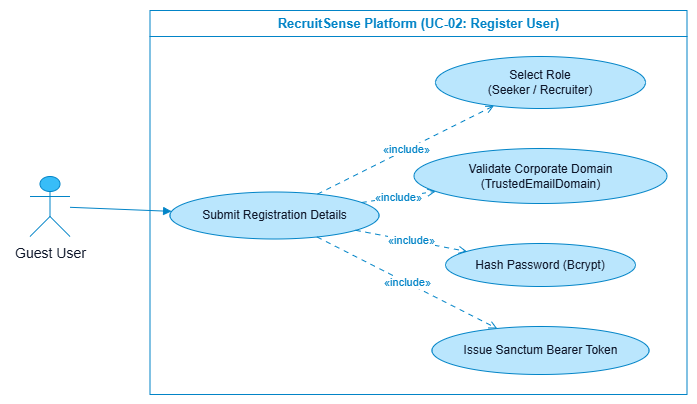
\includegraphics[width=0.65\linewidth]{figures/usecase_register.png}
\caption{Register User with Role Assignment Use Case Diagram}
\label{fig:uc02_diag}
\end{figure}

\begin{table}[H]
\centering
\small
\caption{Use Case: Register User with Role Assignment (UC-02)}
\label{tab:uc02_spec}
\begin{tabular}{|p{3.2cm}|p{5.5cm}|p{5.5cm}|}
\hline
\textbf{Use Case ID:} & \multicolumn{2}{p{11.4cm}|}{UC-02} \\ \hline
\textbf{Use Case Name:} & \multicolumn{2}{p{11.4cm}|}{Register User with Role Assignment} \\ \hline
\textbf{Created By:} & \multicolumn{2}{p{11.4cm}|}{Hamza Zahoor} \\ \hline
\textbf{Last Updated By:} & \multicolumn{2}{p{11.4cm}|}{Haseeb Ahmed} \\ \hline
\textbf{Actors:} & \multicolumn{2}{p{11.4cm}|}{Guest (New User)} \\ \hline
\textbf{Description:} & \multicolumn{2}{p{11.4cm}|}{New user creates an account with role-specific validation and corporate domain verification.} \\ \hline
\textbf{Trigger:} & \multicolumn{2}{p{11.4cm}|}{User clicks ``Sign Up'' on the navigation bar.} \\ \hline
\textbf{Preconditions:} & \multicolumn{2}{p{11.4cm}|}{User possesses a valid, unique email address. \newline User has not previously registered with the same email.} \\ \hline
\textbf{Post conditions:} & \multicolumn{2}{p{11.4cm}|}{User account is created in MySQL database. \newline Sanctum Bearer token is issued and stored in client state.} \\ \hline
\multirow{3}{*}{\textbf{Normal Flow:}} & \multicolumn{1}{c|}{\textbf{Actor}} & \multicolumn{1}{c|}{\textbf{System}} \\ \cline{2-3}
& 1. User enters name, email, password, and selects role. & 2. System validates input formats, password length ($\ge 8$), and domain legitimacy. \vspace{2pt} \\
& 3. User submits registration form. & 4. System hashes password via Bcrypt, inserts record, generates token, and redirects to dashboard. \\ \hline
\textbf{Alternative Flows:} & \multicolumn{2}{p{11.4cm}|}{1. User registers with Google Single Sign-On (OAuth2).} \\ \hline
\textbf{Exceptions:} & \multicolumn{2}{p{11.4cm}|}{1. Email already registered (HTTP 422 Unprocessable Entity returned). \newline 2. Employer email uses blacklisted disposable domain (Registration blocked with explanatory prompt).} \\ \hline
\end{tabular}
\end{table}

\subsection{User Login and Token Authentication (UC-03)}
When a registered user accesses RecruitSense, they authenticate by entering their registered email and password on web or mobile. The Laravel backend verifies credential validity against the database, checks whether the account is active or suspended, generates a cryptographically secure Sanctum personal access token with role-scoped abilities, and returns the token along with user profile metadata. The React web client or Flutter mobile application persists the token securely and mounts the appropriate dashboard based on user role. This workflow is depicted in Figure \ref{fig:uc03_diag} and summarised in Table \ref{tab:uc03_spec}.

\begin{figure}[H]
\centering
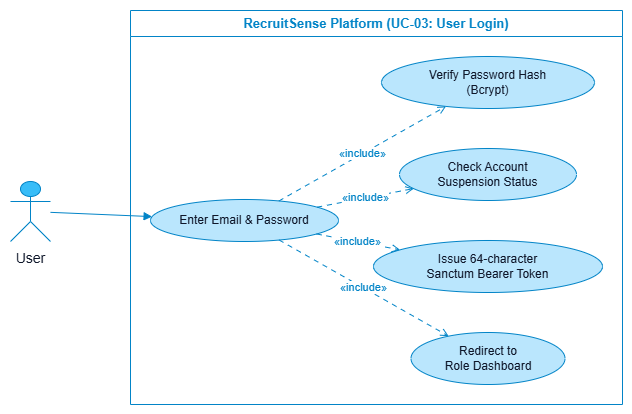
\includegraphics[width=0.65\linewidth]{figures/usecase_login.png}
\caption{User Login and Token Authentication Use Case Diagram}
\label{fig:uc03_diag}
\end{figure}

\begin{table}[H]
\centering
\small
\caption{Use Case: User Login and Token Authentication (UC-03)}
\label{tab:uc03_spec}
\begin{tabular}{|p{3.2cm}|p{5.5cm}|p{5.5cm}|}
\hline
\textbf{Use Case ID:} & \multicolumn{2}{p{11.4cm}|}{UC-03} \\ \hline
\textbf{Use Case Name:} & \multicolumn{2}{p{11.4cm}|}{User Login and Token Authentication} \\ \hline
\textbf{Created By:} & \multicolumn{2}{p{11.4cm}|}{Hamza Zahoor} \\ \hline
\textbf{Last Updated By:} & \multicolumn{2}{p{11.4cm}|}{Haseeb Ahmed} \\ \hline
\textbf{Actors:} & \multicolumn{2}{p{11.4cm}|}{Registered User (Job Seeker, Recruiter, Admin)} \\ \hline
\textbf{Description:} & \multicolumn{2}{p{11.4cm}|}{Authenticate user credentials and establish a secure, tokenized session.} \\ \hline
\textbf{Trigger:} & \multicolumn{2}{p{11.4cm}|}{User clicks ``Login'' and submits credentials.} \\ \hline
\textbf{Preconditions:} & \multicolumn{2}{p{11.4cm}|}{User account exists in the system and is not in suspended status.} \\ \hline
\textbf{Post conditions:} & \multicolumn{2}{p{11.4cm}|}{Sanctum Bearer token generated and user authenticated into role-specific dashboard.} \\ \hline
\multirow{3}{*}{\textbf{Normal Flow:}} & \multicolumn{1}{c|}{\textbf{Actor}} & \multicolumn{1}{c|}{\textbf{System}} \\ \cline{2-3}
& 1. User enters registered email and password. & 2. System validates input syntax and format. \vspace{2pt} \\
& 3. User clicks ``Login''. & 4. System verifies Bcrypt hash, checks account status, issues Sanctum token, and redirects by role. \\ \hline
\textbf{Alternative Flows:} & \multicolumn{2}{p{11.4cm}|}{1. User resets forgotten password via email reset token. \newline 2. User logs in using authenticated Google OAuth token.} \\ \hline
\textbf{Exceptions:} & \multicolumn{2}{p{11.4cm}|}{1. Invalid credentials entered (HTTP 401 Unauthorized error returned). \newline 2. Account is suspended (HTTP 403 Forbidden with support contact info).} \\ \hline
\end{tabular}
\end{table}

\subsection{Create and Publish Job Vacancy (UC-04)}
Corporate recruiters can create and publish new job vacancies through a dedicated posting interface. The recruiter provides the Job Title, Department, Location, Employment Type, Compensation Range, detailed Job Description, Minimum Experience Years, and explicit Required Technical Skills. The system validates all inputs, ensures the employer's company profile is verified, persists the vacancy to MySQL, and immediately publishes the listing to the public job board, making it discoverable to job seekers. This workflow is depicted in Figure \ref{fig:uc04_diag} and summarised in Table \ref{tab:uc04_spec}.

\begin{figure}[H]
\centering
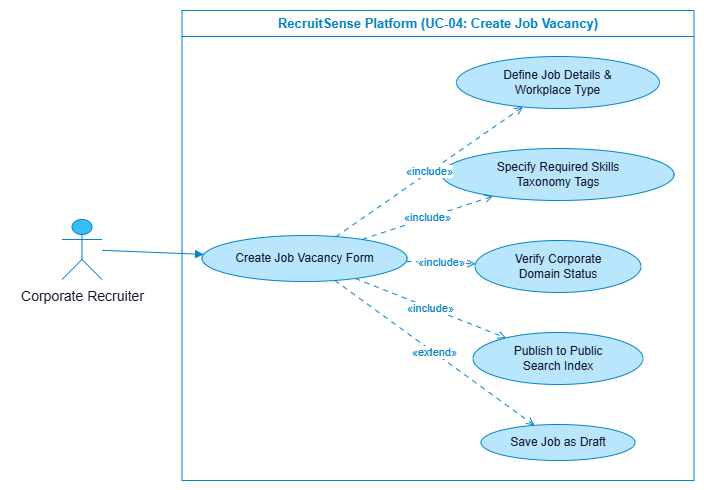
\includegraphics[width=0.65\linewidth]{figures/usecase_post_job.png}
\caption{Create and Publish Job Vacancy Use Case Diagram}
\label{fig:uc04_diag}
\end{figure}

\begin{table}[H]
\centering
\small
\caption{Use Case: Create and Publish Job Vacancy (UC-04)}
\label{tab:uc04_spec}
\begin{tabular}{|p{3.2cm}|p{5.5cm}|p{5.5cm}|}
\hline
\textbf{Use Case ID:} & \multicolumn{2}{p{11.4cm}|}{UC-04} \\ \hline
\textbf{Use Case Name:} & \multicolumn{2}{p{11.4cm}|}{Create and Publish Job Vacancy} \\ \hline
\textbf{Created By:} & \multicolumn{2}{p{11.4cm}|}{Hamza Zahoor} \\ \hline
\textbf{Last Updated By:} & \multicolumn{2}{p{11.4cm}|}{Haseeb Ahmed} \\ \hline
\textbf{Actors:} & \multicolumn{2}{p{11.4cm}|}{Corporate Recruiter / Employer} \\ \hline
\textbf{Description:} & \multicolumn{2}{p{11.4cm}|}{Recruiter defines job details, tags required skills, and publishes an active opening.} \\ \hline
\textbf{Trigger:} & \multicolumn{2}{p{11.4cm}|}{Recruiter clicks ``Post a New Job'' on the recruiter dashboard.} \\ \hline
\textbf{Preconditions:} & \multicolumn{2}{p{11.4cm}|}{Recruiter is authenticated and possesses a verified corporate company profile.} \\ \hline
\textbf{Post conditions:} & \multicolumn{2}{p{11.4cm}|}{A new job record is inserted into the \texttt{job\_postings} table with status \texttt{'active'}.} \\ \hline
\multirow{4}{*}{\textbf{Normal Flow:}} & \multicolumn{1}{c|}{\textbf{Actor}} & \multicolumn{1}{c|}{\textbf{System}} \\ \cline{2-3}
& 1. Recruiter fills out job posting form (title, department, salary, description). & 2. System validates input constraints and corporate posting eligibility. \vspace{2pt} \\
& 3. Recruiter tags required technical skills (e.g., React, Laravel, MySQL). & 4. System parses skill tokens against technology taxonomy. \vspace{2pt} \\
& 5. Recruiter clicks ``Publish Job''. & 6. System persists record, activates listing, and confirms publication. \\ \hline
\textbf{Alternative Flows:} & \multicolumn{2}{p{11.4cm}|}{1. Recruiter saves job as a \texttt{'draft'} for later editing.} \\ \hline
\textbf{Exceptions:} & \multicolumn{2}{p{11.4cm}|}{1. Required fields missing (System displays form validation errors). \newline 2. Company profile is unverified (Posting blocked until domain verification).} \\ \hline
\end{tabular}
\end{table}

\subsection{Submit Job Application with Resume Upload (UC-05)}
When a job seeker discovers a relevant job opening, they submit their application by uploading their resume in PDF format. The backend validates file format and size constraints ($\le 5\text{MB}$), encrypts and stores the file on secure disk storage with an obfuscated UUID filename, and automatically triggers the internal AI screening microservice to parse the document, extract skills, index embeddings into ChromaDB, and calculate the candidate's ATS match score. This workflow is depicted in Figure \ref{fig:uc05_diag} and summarised in Table \ref{tab:uc05_spec}.

\begin{figure}[H]
\centering
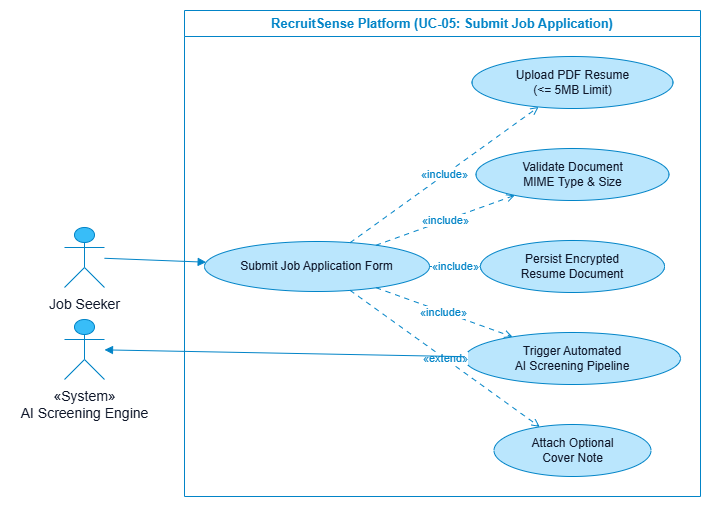
\includegraphics[width=0.65\linewidth]{figures/usecase_apply.png}
\caption{Submit Job Application with Resume Upload Use Case Diagram}
\label{fig:uc05_diag}
\end{figure}

\begin{table}[H]
\centering
\small
\caption{Use Case: Submit Job Application with Resume Upload (UC-05)}
\label{tab:uc05_spec}
\begin{tabular}{|p{3.2cm}|p{5.5cm}|p{5.5cm}|}
\hline
\textbf{Use Case ID:} & \multicolumn{2}{p{11.4cm}|}{UC-05} \\ \hline
\textbf{Use Case Name:} & \multicolumn{2}{p{11.4cm}|}{Submit Job Application with Resume Upload} \\ \hline
\textbf{Created By:} & \multicolumn{2}{p{11.4cm}|}{Hamza Zahoor} \\ \hline
\textbf{Last Updated By:} & \multicolumn{2}{p{11.4cm}|}{Haseeb Ahmed} \\ \hline
\textbf{Actors:} & \multicolumn{2}{p{11.4cm}|}{Job Seeker} \\ \hline
\textbf{Description:} & \multicolumn{2}{p{11.4cm}|}{Candidate submits an application with PDF resume upload triggering automated screening.} \\ \hline
\textbf{Trigger:} & \multicolumn{2}{p{11.4cm}|}{Candidate clicks ``Apply Now'' on a job details modal.} \\ \hline
\textbf{Preconditions:} & \multicolumn{2}{p{11.4cm}|}{Candidate is authenticated into an active Job Seeker account. \newline Target job vacancy is active and accepting applications.} \\ \hline
\textbf{Post conditions:} & \multicolumn{2}{p{11.4cm}|}{Application record created in database; resume stored; ATS screening triggered.} \\ \hline
\multirow{3}{*}{\textbf{Normal Flow:}} & \multicolumn{1}{c|}{\textbf{Actor}} & \multicolumn{1}{c|}{\textbf{System}} \\ \cline{2-3}
& 1. Candidate selects resume file (PDF) and enters optional cover note. & 2. System verifies PDF MIME type and ensures file size $\le 5\text{MB}$. \vspace{2pt} \\
& 3. Candidate clicks ``Submit Application''. & 4. System writes file to disk, dispatches payload to FastAPI AI service, persists calculated ATS score, and renders confirmation. \\ \hline
\textbf{Alternative Flows:} & \multicolumn{2}{p{11.4cm}|}{1. Candidate uses previously uploaded profile resume.} \\ \hline
\textbf{Exceptions:} & \multicolumn{2}{p{11.4cm}|}{1. File exceeds 5MB or invalid extension (HTTP 422 error). \newline 2. Candidate has already applied to this posting (Duplicate prevention).} \\ \hline
\end{tabular}
\end{table}

\subsection{Automated AI Resume Parsing and Semantic ATS Screening (UC-06)}
As an autonomous system actor, the Python FastAPI AI microservice receives the binary resume stream and job vacancy criteria from the Laravel backend. It extracts the raw text stream using PyPDF2, sanitizes punctuation and whitespace, executes boundary-delimited regex matching against required and bonus skill dictionaries, generates dense vector embeddings, and indexes chunks into ChromaDB for Candidate RAG retrieval. The structured evaluation is returned as JSON to the backend. This workflow is depicted in Figure \ref{fig:uc06_diag} and summarised in Table \ref{tab:uc06_spec}.

\begin{figure}[H]
\centering
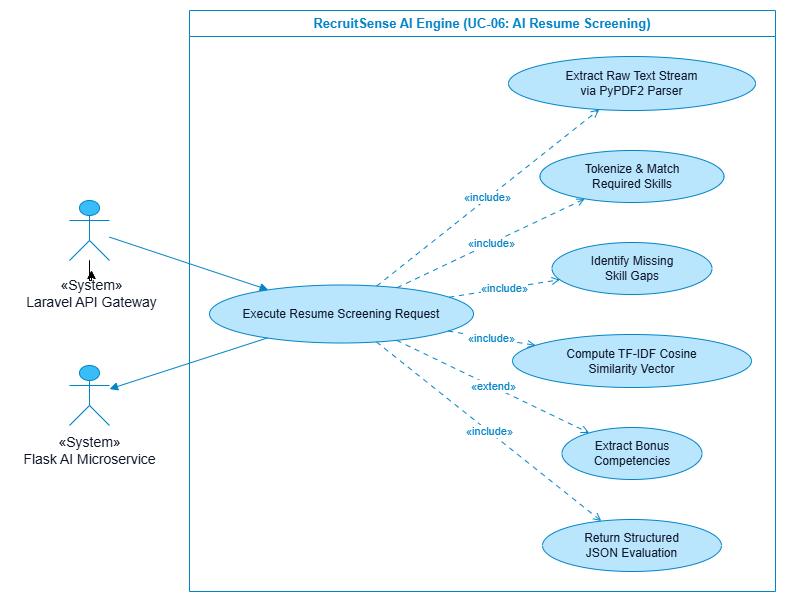
\includegraphics[width=0.65\linewidth]{figures/usecase_ai_screening.png}
\caption{Automated AI Resume Parsing and Semantic ATS Screening Use Case Diagram}
\label{fig:uc06_diag}
\end{figure}

\begin{table}[H]
\centering
\small
\caption{Use Case: Automated AI Resume Parsing and Semantic ATS Screening (UC-06)}
\label{tab:uc06_spec}
\begin{tabular}{|p{3.2cm}|p{5.5cm}|p{5.5cm}|}
\hline
\textbf{Use Case ID:} & \multicolumn{2}{p{11.4cm}|}{UC-06} \\ \hline
\textbf{Use Case Name:} & \multicolumn{2}{p{11.4cm}|}{Automated AI Resume Parsing and Semantic ATS Screening} \\ \hline
\textbf{Created By:} & \multicolumn{2}{p{11.4cm}|}{Hamza Zahoor} \\ \hline
\textbf{Last Updated By:} & \multicolumn{2}{p{11.4cm}|}{Haseeb Ahmed} \\ \hline
\textbf{Actors:} & \multicolumn{2}{p{11.4cm}|}{AI Screening Microservice (System Actor)} \\ \hline
\textbf{Description:} & \multicolumn{2}{p{11.4cm}|}{Autonomous microservice processes PDF text, extracts skills, and indexes embeddings into ChromaDB.} \\ \hline
\textbf{Trigger:} & \multicolumn{2}{p{11.4cm}|}{Laravel backend sends HTTP POST request to AI microservice.} \\ \hline
\textbf{Preconditions:} & \multicolumn{2}{p{11.4cm}|}{Valid PDF stream and job description strings provided in payload.} \\ \hline
\textbf{Post conditions:} & \multicolumn{2}{p{11.4cm}|}{Structured JSON evaluation returned containing scores, matched skills, and skill gaps.} \\ \hline
\multirow{3}{*}{\textbf{Normal Flow:}} & \multicolumn{1}{c|}{\textbf{Actor}} & \multicolumn{1}{c|}{\textbf{System}} \\ \cline{2-3}
& 1. Backend dispatches multipart request with resume and required skills. & 2. AI Service extracts raw text from PDF and matches required skills against taxonomy. \vspace{2pt} \\
& 3. Backend receives structured JSON scoring payload. & 4. AI Service generates dense vector embeddings and indexes document chunks into ChromaDB. \\ \hline
\textbf{Alternative Flows:} & \multicolumn{2}{p{11.4cm}|}{1. AI service extracts bonus skills outside the required skills list.} \\ \hline
\textbf{Exceptions:} & \multicolumn{2}{p{11.4cm}|}{1. PDF has no extractable text layer (HTTP 422 error returned). \newline 2. Memory limit exceeded on oversized documents.} \\ \hline
\end{tabular}
\end{table}

\subsection{View ATS Match Diagnostics and Skill Gap Analysis (UC-07)}
Job seekers and recruiters can view granular, transparent ATS evaluation breakdowns for any submitted application. The web interface displays the overall ATS Match Percentage, a visual gauge, a green badge list of verified matched skills, a red badge list of identified missing skills, and bonus competencies. This eliminates the ATS black box and provides candidates with clear career development feedback. This workflow is depicted in Figure \ref{fig:uc07_diag} and summarised in Table \ref{tab:uc07_spec}.

\begin{figure}[H]
\centering
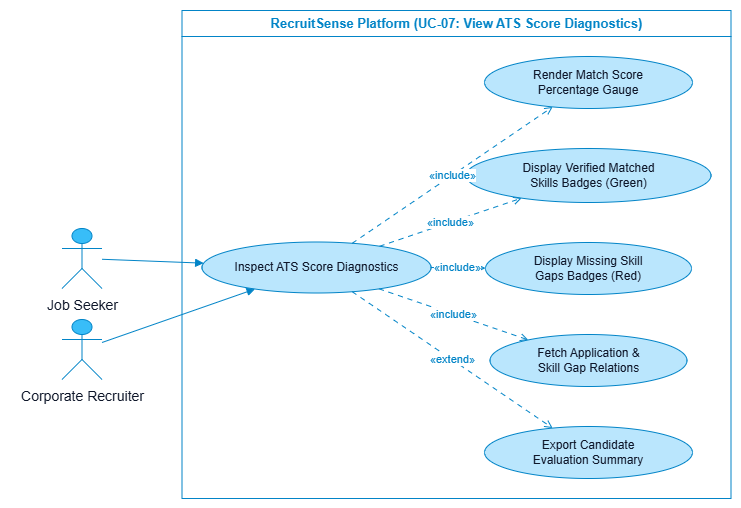
\includegraphics[width=0.65\linewidth]{figures/usecase_ats_score.png}
\caption{View ATS Match Diagnostics and Skill Gap Analysis Use Case Diagram}
\label{fig:uc07_diag}
\end{figure}

\begin{table}[H]
\centering
\small
\caption{Use Case: View ATS Match Diagnostics and Skill Gap Analysis (UC-07)}
\label{tab:uc07_spec}
\begin{tabular}{|p{3.2cm}|p{5.5cm}|p{5.5cm}|}
\hline
\textbf{Use Case ID:} & \multicolumn{2}{p{11.4cm}|}{UC-07} \\ \hline
\textbf{Use Case Name:} & \multicolumn{2}{p{11.4cm}|}{View ATS Match Diagnostics and Skill Gap Analysis} \\ \hline
\textbf{Created By:} & \multicolumn{2}{p{11.4cm}|}{Hamza Zahoor} \\ \hline
\textbf{Last Updated By:} & \multicolumn{2}{p{11.4cm}|}{Haseeb Ahmed} \\ \hline
\textbf{Actors:} & \multicolumn{2}{p{11.4cm}|}{Job Seeker, Corporate Recruiter} \\ \hline
\textbf{Description:} & \multicolumn{2}{p{11.4cm}|}{Display comprehensive ATS score breakdown, matched skills, and missing skill badges.} \\ \hline
\textbf{Trigger:} & \multicolumn{2}{p{11.4cm}|}{User clicks ``View ATS Breakdown'' on an application card.} \\ \hline
\textbf{Preconditions:} & \multicolumn{2}{p{11.4cm}|}{Application exists and has been screened by the AI engine.} \\ \hline
\textbf{Post conditions:} & \multicolumn{2}{p{11.4cm}|}{Diagnostic score modal is rendered with color-coded skill badges.} \\ \hline
\multirow{3}{*}{\textbf{Normal Flow:}} & \multicolumn{1}{c|}{\textbf{Actor}} & \multicolumn{1}{c|}{\textbf{System}} \\ \cline{2-3}
& 1. User navigates to application details. & 2. System retrieves application record and associated \texttt{skill\_gaps} data. \vspace{2pt} \\
& 3. User inspects individual matched and missing skill chips. & 4. System renders overall match percentage, matched skills (green), and missing skills (red). \\ \hline
\textbf{Alternative Flows:} & \multicolumn{2}{p{11.4cm}|}{1. Recruiter downloads extracted candidate summary report.} \\ \hline
\textbf{Exceptions:} & \multicolumn{2}{p{11.4cm}|}{1. Application is pending asynchronous screening calculation.} \\ \hline
\end{tabular}
\end{table}

\subsection{Review AI-Ranked Candidate Shortlist (UC-08)}
Recruiters can inspect all applications received for a particular job vacancy, automatically sorted in descending order of calculated ATS Match Score. Recruiters can apply threshold filters (e.g., show only candidates with $\ge 80\%$ match), inspect extracted resume texts, compare applicant skill distributions, and identify top talent within seconds. This workflow is depicted in Figure \ref{fig:uc08_diag} and summarised in Table \ref{tab:uc08_spec}.

\begin{figure}[H]
\centering
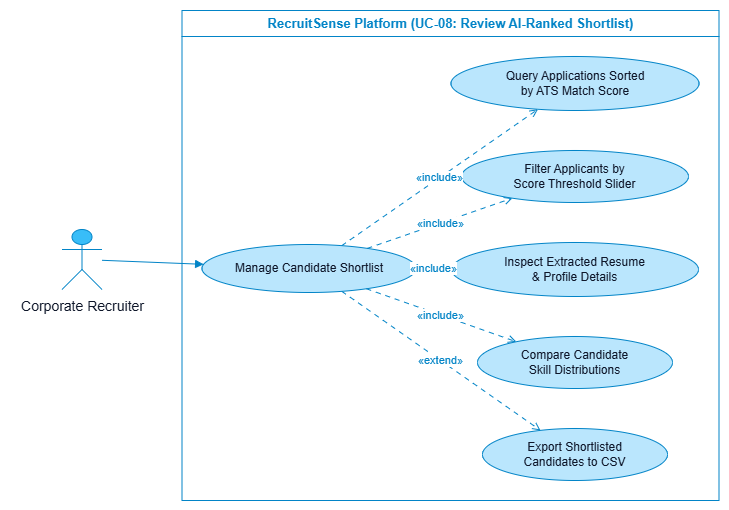
\includegraphics[width=0.65\linewidth]{figures/usecase_shortlist.png}
\caption{Review AI-Ranked Candidate Shortlist Use Case Diagram}
\label{fig:uc08_diag}
\end{figure}

\begin{table}[H]
\centering
\small
\caption{Use Case: Review AI-Ranked Candidate Shortlist (UC-08)}
\label{tab:uc08_spec}
\begin{tabular}{|p{3.2cm}|p{5.5cm}|p{5.5cm}|}
\hline
\textbf{Use Case ID:} & \multicolumn{2}{p{11.4cm}|}{UC-08} \\ \hline
\textbf{Use Case Name:} & \multicolumn{2}{p{11.4cm}|}{Review AI-Ranked Candidate Shortlist} \\ \hline
\textbf{Created By:} & \multicolumn{2}{p{11.4cm}|}{Hamza Zahoor} \\ \hline
\textbf{Last Updated By:} & \multicolumn{2}{p{11.4cm}|}{Haseeb Ahmed} \\ \hline
\textbf{Actors:} & \multicolumn{2}{p{11.4cm}|}{Corporate Recruiter / Employer} \\ \hline
\textbf{Description:} & \multicolumn{2}{p{11.4cm}|}{Recruiter reviews candidate applications sorted by AI match score with filter controls.} \\ \hline
\textbf{Trigger:} & \multicolumn{2}{p{11.4cm}|}{Recruiter selects ``Manage Applicants'' for an active job posting.} \\ \hline
\textbf{Preconditions:} & \multicolumn{2}{p{11.4cm}|}{Recruiter is authenticated; job posting has received at least one application.} \\ \hline
\textbf{Post conditions:} & \multicolumn{2}{p{11.4cm}|}{Tabular candidate ranking list is displayed with score metrics.} \\ \hline
\multirow{4}{*}{\textbf{Normal Flow:}} & \multicolumn{1}{c|}{\textbf{Actor}} & \multicolumn{1}{c|}{\textbf{System}} \\ \cline{2-3}
& 1. Recruiter selects job posting. & 2. System queries \texttt{applications} joined with \texttt{job\_seekers}, sorted by \texttt{ats\_score DESC}. \vspace{2pt} \\
& 3. Recruiter adjusts minimum score slider (e.g., $75\%$). & 4. System filters list dynamically without full page reload. \vspace{2pt} \\
& 5. Recruiter clicks on top-ranked candidate profile. & 6. System displays detailed candidate profile and resume preview. \\ \hline
\textbf{Alternative Flows:} & \multicolumn{2}{p{11.4cm}|}{1. Recruiter exports shortlisted candidate table to CSV.} \\ \hline
\textbf{Exceptions:} & \multicolumn{2}{p{11.4cm}|}{1. Job posting has received zero applicants (System displays friendly empty state).} \\ \hline
\end{tabular}
\end{table}

\subsection{Manage Hiring Pipeline Status (UC-09)}
Recruiters can transition candidate applications through the hiring stages (\textit{Applied} $\rightarrow$ \textit{Screening} $\rightarrow$ \textit{Shortlisted} $\rightarrow$ \textit{Interview Scheduled} $\rightarrow$ \textit{Offer Extended} $\rightarrow$ \textit{Accepted / Rejected}). Changing status immediately updates the candidate's tracking dashboard and triggers automated notification alerts. This workflow is depicted in Figure \ref{fig:uc09_diag} and summarised in Table \ref{tab:uc09_spec}.

\begin{figure}[H]
\centering
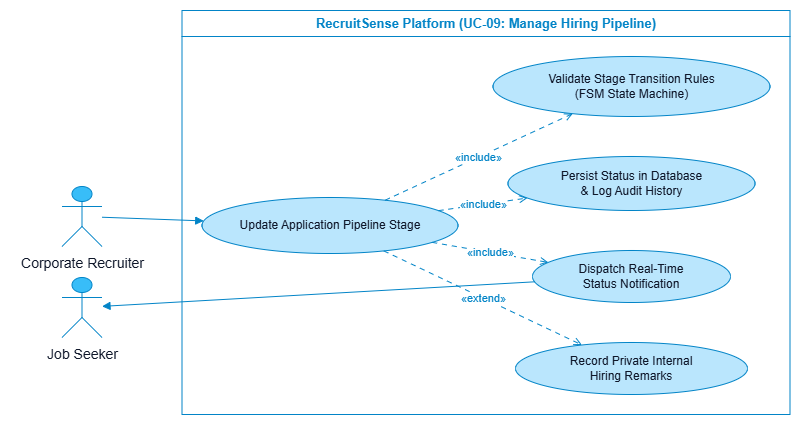
\includegraphics[width=0.65\linewidth]{figures/usecase_pipeline.png}
\caption{Manage Hiring Pipeline Status Use Case Diagram}
\label{fig:uc09_diag}
\end{figure}

\begin{table}[H]
\centering
\small
\caption{Use Case: Manage Hiring Pipeline Status (UC-09)}
\label{tab:uc09_spec}
\begin{tabular}{|p{3.2cm}|p{5.5cm}|p{5.5cm}|}
\hline
\textbf{Use Case ID:} & \multicolumn{2}{p{11.4cm}|}{UC-09} \\ \hline
\textbf{Use Case Name:} & \multicolumn{2}{p{11.4cm}|}{Manage Hiring Pipeline Status} \\ \hline
\textbf{Created By:} & \multicolumn{2}{p{11.4cm}|}{Hamza Zahoor} \\ \hline
\textbf{Last Updated By:} & \multicolumn{2}{p{11.4cm}|}{Haseeb Ahmed} \\ \hline
\textbf{Actors:} & \multicolumn{2}{p{11.4cm}|}{Corporate Recruiter / Employer} \\ \hline
\textbf{Description:} & \multicolumn{2}{p{11.4cm}|}{Recruiter advances candidate applications across hiring funnel stages.} \\ \hline
\textbf{Trigger:} & \multicolumn{2}{p{11.4cm}|}{Recruiter changes the status dropdown on an applicant card.} \\ \hline
\textbf{Preconditions:} & \multicolumn{2}{p{11.4cm}|}{Recruiter is authenticated and owns the job posting associated with the application.} \\ \hline
\textbf{Post conditions:} & \multicolumn{2}{p{11.4cm}|}{Application status is updated in MySQL; notification event dispatched.} \\ \hline
\multirow{3}{*}{\textbf{Normal Flow:}} & \multicolumn{1}{c|}{\textbf{Actor}} & \multicolumn{1}{c|}{\textbf{System}} \\ \cline{2-3}
& 1. Recruiter selects new stage (e.g., \textit{Shortlisted} or \textit{Interview Scheduled}). & 2. System validates transition validity against hiring FSM rules. \vspace{2pt} \\
& 3. Recruiter confirms stage update. & 4. System updates \texttt{applications.status}, logs audit history, and sends candidate notification. \\ \hline
\textbf{Alternative Flows:} & \multicolumn{2}{p{11.4cm}|}{1. Recruiter enters internal hiring remarks visible only to company staff.} \\ \hline
\textbf{Exceptions:} & \multicolumn{2}{p{11.4cm}|}{1. Candidate has withdrawn application (Status change blocked).} \\ \hline
\end{tabular}
\end{table}

\subsection{Edit and Update Job Vacancy (UC-10)}
Recruiters can modify details of existing job postings (e.g., updating salary range, revising required skills, or extending application deadlines). The system loads current data, validates updates, persists changes, and logs modifications for auditing. This workflow is depicted in Figure \ref{fig:uc10_diag} and summarised in Table \ref{tab:uc10_spec}.

\begin{figure}[H]
\centering
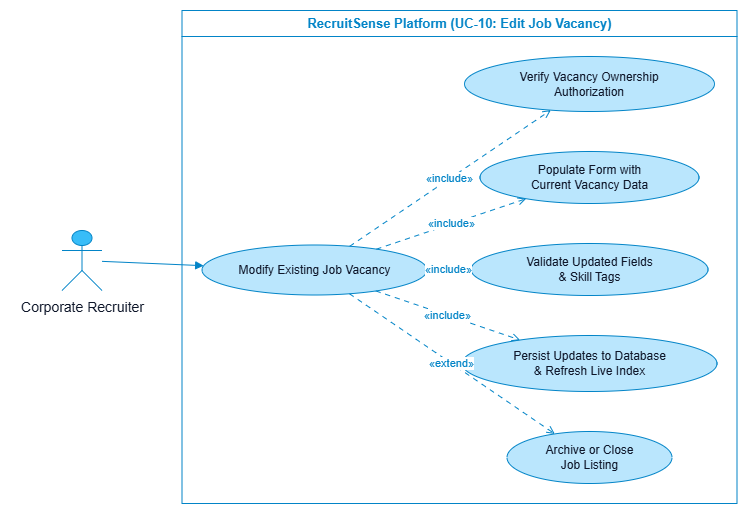
\includegraphics[width=0.65\linewidth]{figures/usecase_edit_job.png}
\caption{Edit and Update Job Vacancy Use Case Diagram}
\label{fig:uc10_diag}
\end{figure}

\begin{table}[H]
\centering
\small
\caption{Use Case: Edit and Update Job Vacancy (UC-10)}
\label{tab:uc10_spec}
\begin{tabular}{|p{3.2cm}|p{5.5cm}|p{5.5cm}|}
\hline
\textbf{Use Case ID:} & \multicolumn{2}{p{11.4cm}|}{UC-10} \\ \hline
\textbf{Use Case Name:} & \multicolumn{2}{p{11.4cm}|}{Edit and Update Job Vacancy} \\ \hline
\textbf{Created By:} & \multicolumn{2}{p{11.4cm}|}{Hamza Zahoor} \\ \hline
\textbf{Last Updated By:} & \multicolumn{2}{p{11.4cm}|}{Haseeb Ahmed} \\ \hline
\textbf{Actors:} & \multicolumn{2}{p{11.4cm}|}{Corporate Recruiter / Employer} \\ \hline
\textbf{Description:} & \multicolumn{2}{p{11.4cm}|}{Recruiter modifies information, requirements, or status of an existing job posting.} \\ \hline
\textbf{Trigger:} & \multicolumn{2}{p{11.4cm}|}{Recruiter clicks ``Edit'' on an active or draft job posting.} \\ \hline
\textbf{Preconditions:} & \multicolumn{2}{p{11.4cm}|}{Recruiter is authenticated and owns the job posting.} \\ \hline
\textbf{Post conditions:} & \multicolumn{2}{p{11.4cm}|}{Job posting data updated in MySQL; live listing refreshed.} \\ \hline
\multirow{4}{*}{\textbf{Normal Flow:}} & \multicolumn{1}{c|}{\textbf{Actor}} & \multicolumn{1}{c|}{\textbf{System}} \\ \cline{2-3}
& 1. Recruiter selects job to edit. & 2. System populates editable form with current record. \vspace{2pt} \\
& 3. Recruiter modifies description, salary, or required skills. & 4. System validates modified fields and input constraints. \vspace{2pt} \\
& 5. Recruiter clicks ``Save Changes''. & 6. System updates \texttt{job\_postings} table and refreshes listing view. \\ \hline
\textbf{Alternative Flows:} & \multicolumn{2}{p{11.4cm}|}{1. Recruiter closes or archives the job posting.} \\ \hline
\textbf{Exceptions:} & \multicolumn{2}{p{11.4cm}|}{1. Unauthorized edit attempt by non-owner recruiter (HTTP 403 Forbidden).} \\ \hline
\end{tabular}
\end{table}

\subsection{Save Job to Bookmarks (UC-11)}
Job seekers can bookmark vacancies of interest into a personalized ``Saved Jobs'' list, enabling easy access and application preparation. Clicking the bookmark button persists the bookmark to the database, toggles the visual icon, and adds the listing to the candidate's saved vacancies view. This workflow is depicted in Figure \ref{fig:uc11_diag} and summarised in Table \ref{tab:uc11_spec}.

\begin{figure}[H]
\centering
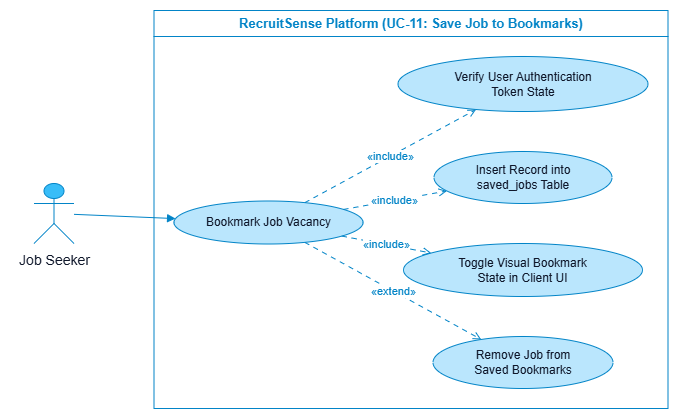
\includegraphics[width=0.65\linewidth]{figures/usecase_save_job.png}
\caption{Save Job to Bookmarks Use Case Diagram}
\label{fig:uc11_diag}
\end{figure}

\begin{table}[H]
\centering
\small
\caption{Use Case: Save Job to Bookmarks (UC-11)}
\label{tab:uc11_spec}
\begin{tabular}{|p{3.2cm}|p{5.5cm}|p{5.5cm}|}
\hline
\textbf{Use Case ID:} & \multicolumn{2}{p{11.4cm}|}{UC-11} \\ \hline
\textbf{Use Case Name:} & \multicolumn{2}{p{11.4cm}|}{Save Job to Bookmarks} \\ \hline
\textbf{Created By:} & \multicolumn{2}{p{11.4cm}|}{Hamza Zahoor} \\ \hline
\textbf{Last Updated By:} & \multicolumn{2}{p{11.4cm}|}{Haseeb Ahmed} \\ \hline
\textbf{Actors:} & \multicolumn{2}{p{11.4cm}|}{Job Seeker} \\ \hline
\textbf{Description:} & \multicolumn{2}{p{11.4cm}|}{Candidate bookmarks a job listing for future review and tracking.} \\ \hline
\textbf{Trigger:} & \multicolumn{2}{p{11.4cm}|}{Candidate clicks the bookmark icon on any job card.} \\ \hline
\textbf{Preconditions:} & \multicolumn{2}{p{11.4cm}|}{Candidate is logged into an active Job Seeker account.} \\ \hline
\textbf{Post conditions:} & \multicolumn{2}{p{11.4cm}|}{Record inserted into \texttt{saved\_jobs} table; UI badge toggled.} \\ \hline
\multirow{3}{*}{\textbf{Normal Flow:}} & \multicolumn{1}{c|}{\textbf{Actor}} & \multicolumn{1}{c|}{\textbf{System}} \\ \cline{2-3}
& 1. Candidate clicks bookmark icon on a job card. & 2. System verifies authentication and inserts record into \texttt{saved\_jobs} table. \vspace{2pt} \\
& 3. Candidate navigates to Saved Jobs workspace. & 4. System renders bookmarked vacancies in candidate dashboard. \\ \hline
\textbf{Alternative Flows:} & \multicolumn{2}{p{11.4cm}|}{1. Candidate clicks bookmark icon again to remove job from saved list.} \\ \hline
\textbf{Exceptions:} & \multicolumn{2}{p{11.4cm}|}{1. Unauthenticated user clicks bookmark (System prompts login modal).} \\ \hline
\end{tabular}
\end{table}

\subsection{Real-Time In-App Messaging (UC-12)}
Job seekers and corporate recruiters can communicate directly within the platform regarding job inquiries, interview details, and hiring coordination. All messages are securely sanitized against XSS vulnerabilities, persisted to MySQL, and delivered with real-time UI synchronization. This workflow is depicted in Figure \ref{fig:uc12_diag} and summarised in Table \ref{tab:uc12_spec}.

\begin{figure}[H]
\centering
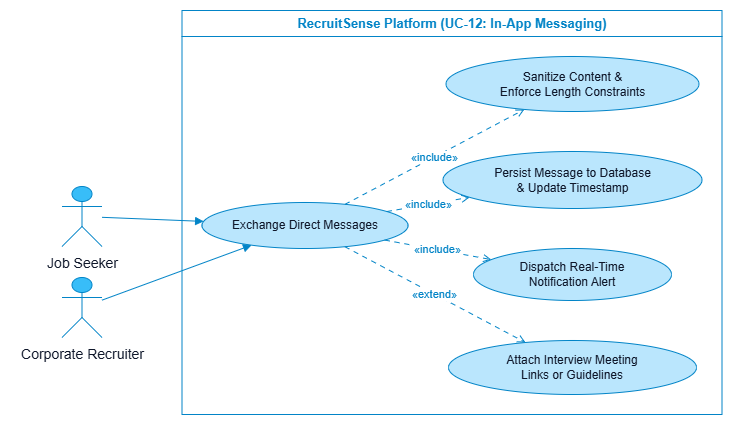
\includegraphics[width=0.65\linewidth]{figures/usecase_message.png}
\caption{Real-Time In-App Messaging Use Case Diagram}
\label{fig:uc12_diag}
\end{figure}

\begin{table}[H]
\centering
\small
\caption{Use Case: Real-Time In-App Messaging (UC-12)}
\label{tab:uc12_spec}
\begin{tabular}{|p{3.2cm}|p{5.5cm}|p{5.5cm}|}
\hline
\textbf{Use Case ID:} & \multicolumn{2}{p{11.4cm}|}{UC-12} \\ \hline
\textbf{Use Case Name:} & \multicolumn{2}{p{11.4cm}|}{Real-Time In-App Messaging} \\ \hline
\textbf{Created By:} & \multicolumn{2}{p{11.4cm}|}{Hamza Zahoor} \\ \hline
\textbf{Last Updated By:} & \multicolumn{2}{p{11.4cm}|}{Haseeb Ahmed} \\ \hline
\textbf{Actors:} & \multicolumn{2}{p{11.4cm}|}{Job Seeker, Corporate Recruiter} \\ \hline
\textbf{Description:} & \multicolumn{2}{p{11.4cm}|}{Send and receive direct messages regarding applications and interviews.} \\ \hline
\textbf{Trigger:} & \multicolumn{2}{p{11.4cm}|}{User clicks ``Message'' on candidate profile or job application.} \\ \hline
\textbf{Preconditions:} & \multicolumn{2}{p{11.4cm}|}{Both users are authenticated; an active application context exists.} \\ \hline
\textbf{Post conditions:} & \multicolumn{2}{p{11.4cm}|}{Message persisted in database; recipient notified in real time.} \\ \hline
\multirow{3}{*}{\textbf{Normal Flow:}} & \multicolumn{1}{c|}{\textbf{Actor}} & \multicolumn{1}{c|}{\textbf{System}} \\ \cline{2-3}
& 1. User selects recipient and composes message. & 2. System sanitizes message content against XSS vulnerabilities. \vspace{2pt} \\
& 3. User clicks ``Send''. & 4. System stores message in \texttt{messages} table, updates conversation timestamp, and alerts recipient. \\ \hline
\textbf{Alternative Flows:} & \multicolumn{2}{p{11.4cm}|}{1. Recruiter attaches interview guidelines or document links.} \\ \hline
\textbf{Exceptions:} & \multicolumn{2}{p{11.4cm}|}{1. Message exceeds maximum character limit. \newline 2. User account has been suspended.} \\ \hline
\end{tabular}
\end{table}

\subsection{Schedule Candidate Interview (UC-13)}
When a candidate is moved to the \textit{Interview Scheduled} stage, the recruiter can set the interview date, time, format (In-Person or Virtual), meeting link, and candidate preparation instructions. The system verifies that the scheduled date is in the future, updates the database, and dispatches an instant notification to the candidate. This workflow is depicted in Figure \ref{fig:uc13_diag} and summarised in Table \ref{tab:uc13_spec}.

\begin{figure}[H]
\centering
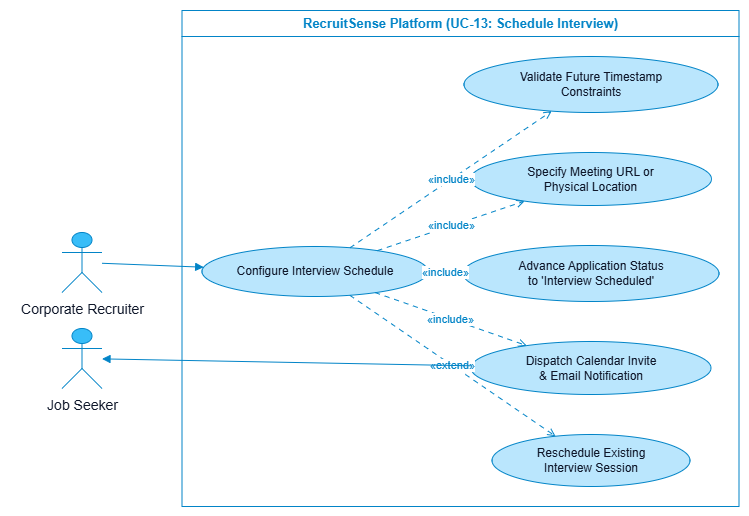
\includegraphics[width=0.65\linewidth]{figures/usecase_interview.png}
\caption{Schedule Candidate Interview Use Case Diagram}
\label{fig:uc13_diag}
\end{figure}

\begin{table}[H]
\centering
\small
\caption{Use Case: Schedule Candidate Interview (UC-13)}
\label{tab:uc13_spec}
\begin{tabular}{|p{3.2cm}|p{5.5cm}|p{5.5cm}|}
\hline
\textbf{Use Case ID:} & \multicolumn{2}{p{11.4cm}|}{UC-13} \\ \hline
\textbf{Use Case Name:} & \multicolumn{2}{p{11.4cm}|}{Schedule Candidate Interview} \\ \hline
\textbf{Created By:} & \multicolumn{2}{p{11.4cm}|}{Hamza Zahoor} \\ \hline
\textbf{Last Updated By:} & \multicolumn{2}{p{11.4cm}|}{Haseeb Ahmed} \\ \hline
\textbf{Actors:} & \multicolumn{2}{p{11.4cm}|}{Corporate Recruiter / Employer} \\ \hline
\textbf{Description:} & \multicolumn{2}{p{11.4cm}|}{Recruiter configures interview schedule, meeting location, and candidate instructions.} \\ \hline
\textbf{Trigger:} & \multicolumn{2}{p{11.4cm}|}{Recruiter selects ``Schedule Interview'' on a shortlisted applicant card.} \\ \hline
\textbf{Preconditions:} & \multicolumn{2}{p{11.4cm}|}{Candidate application is in \textit{Shortlisted} or \textit{Interview} status.} \\ \hline
\textbf{Post conditions:} & \multicolumn{2}{p{11.4cm}|}{\texttt{interview\_at} and \texttt{interview\_location} saved; candidate notified.} \\ \hline
\multirow{4}{*}{\textbf{Normal Flow:}} & \multicolumn{1}{c|}{\textbf{Actor}} & \multicolumn{1}{c|}{\textbf{System}} \\ \cline{2-3}
& 1. Recruiter selects date and time for interview. & 2. System validates date is set in the future. \vspace{2pt} \\
& 3. Recruiter specifies meeting URL (e.g., Google Meet / Teams) or physical address. & 4. System sanitizes location and instructions text. \vspace{2pt} \\
& 5. Recruiter clicks ``Confirm Schedule''. & 6. System updates application record, advances status to \textit{Interview Scheduled}, and dispatches notification. \\ \hline
\textbf{Alternative Flows:} & \multicolumn{2}{p{11.4cm}|}{1. Recruiter reschedules an existing interview date.} \\ \hline
\textbf{Exceptions:} & \multicolumn{2}{p{11.4cm}|}{1. Past date selected (Validation error displayed).} \\ \hline
\end{tabular}
\end{table}

\subsection{Verify Corporate Email Domain (UC-14)}
To prevent fraudulent employers and fake postings, the system validates recruiter email domains during registration and profile creation. Platform administrators can also manually inspect and verify employer organizations, ensuring high platform credibility. This workflow is depicted in Figure \ref{fig:uc14_diag} and summarised in Table \ref{tab:uc14_spec}.

\begin{figure}[H]
\centering
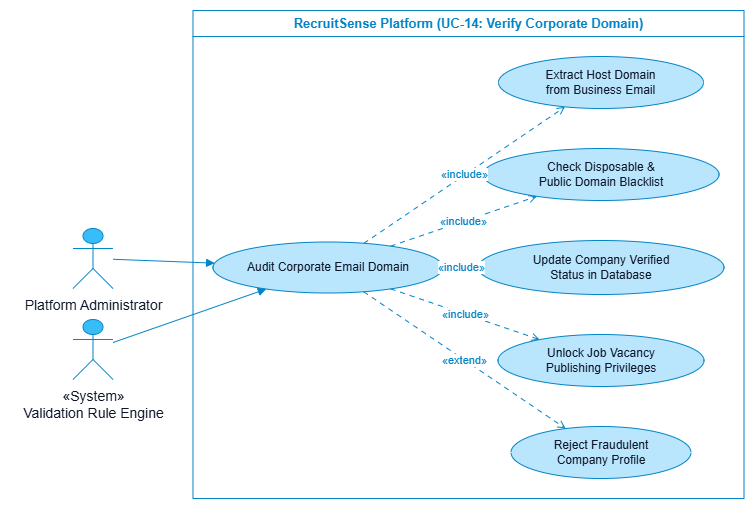
\includegraphics[width=0.65\linewidth]{figures/usecase_domain_verify.png}
\caption{Verify Corporate Email Domain Use Case Diagram}
\label{fig:uc14_diag}
\end{figure}

\begin{table}[H]
\centering
\small
\caption{Use Case: Verify Corporate Email Domain (UC-14)}
\label{tab:uc14_spec}
\begin{tabular}{|p{3.2cm}|p{5.5cm}|p{5.5cm}|}
\hline
\textbf{Use Case ID:} & \multicolumn{2}{p{11.4cm}|}{UC-14} \\ \hline
\textbf{Use Case Name:} & \multicolumn{2}{p{11.4cm}|}{Verify Corporate Email Domain} \\ \hline
\textbf{Created By:} & \multicolumn{2}{p{11.4cm}|}{Hamza Zahoor} \\ \hline
\textbf{Last Updated By:} & \multicolumn{2}{p{11.4cm}|}{Haseeb Ahmed} \\ \hline
\textbf{Actors:} & \multicolumn{2}{p{11.4cm}|}{Administrator, Validation Engine} \\ \hline
\textbf{Description:} & \multicolumn{2}{p{11.4cm}|}{Verify legitimacy of corporate employer email domains and activate posting privileges.} \\ \hline
\textbf{Trigger:} & \multicolumn{2}{p{11.4cm}|}{Recruiter registers or administrator reviews company pending queue.} \\ \hline
\textbf{Preconditions:} & \multicolumn{2}{p{11.4cm}|}{Recruiter has submitted company registration details.} \\ \hline
\textbf{Post conditions:} & \multicolumn{2}{p{11.4cm}|}{\texttt{companies.verified} flag set to \texttt{true}; verified badge displayed.} \\ \hline
\multirow{3}{*}{\textbf{Normal Flow:}} & \multicolumn{1}{c|}{\textbf{Actor}} & \multicolumn{1}{c|}{\textbf{System}} \\ \cline{2-3}
& 1. Recruiter submits registration with business email. & 2. System extracts domain and checks against disposable domain blacklists. \vspace{2pt} \\
& 3. Administrator reviews corporate website and registration details. & 4. System sets \texttt{verified = true} and unlocks job publishing capabilities. \\ \hline
\textbf{Alternative Flows:} & \multicolumn{2}{p{11.4cm}|}{1. Admin rejects fraudulent company profile with explanation.} \\ \hline
\textbf{Exceptions:} & \multicolumn{2}{p{11.4cm}|}{1. Recruiter registered with generic disposable email (System flags profile).} \\ \hline
\end{tabular}
\end{table}

\subsection{Moderate Employer Accounts (UC-15)}
Administrators review pending or reported employer accounts to ensure compliance with recruitment guidelines and fair hiring practices. The administrator can inspect company metrics, verify corporate details, and approve or suspend posting privileges. This workflow is depicted in Figure \ref{fig:uc15_diag} and summarised in Table \ref{tab:uc15_spec}.

\begin{figure}[H]
\centering
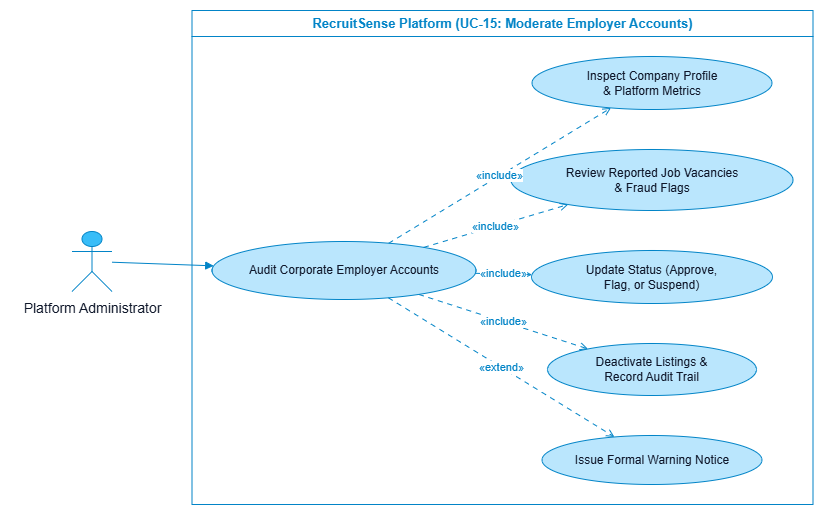
\includegraphics[width=0.65\linewidth]{figures/usecase_moderate_employer.png}
\caption{Moderate Employer Accounts Use Case Diagram}
\label{fig:uc15_diag}
\end{figure}

\begin{table}[H]
\centering
\small
\caption{Use Case: Moderate Employer Accounts (UC-15)}
\label{tab:uc15_spec}
\begin{tabular}{|p{3.2cm}|p{5.5cm}|p{5.5cm}|}
\hline
\textbf{Use Case ID:} & \multicolumn{2}{p{11.4cm}|}{UC-15} \\ \hline
\textbf{Use Case Name:} & \multicolumn{2}{p{11.4cm}|}{Moderate Employer Accounts} \\ \hline
\textbf{Created By:} & \multicolumn{2}{p{11.4cm}|}{Hamza Zahoor} \\ \hline
\textbf{Last Updated By:} & \multicolumn{2}{p{11.4cm}|}{Haseeb Ahmed} \\ \hline
\textbf{Actors:} & \multicolumn{2}{p{11.4cm}|}{Platform Administrator} \\ \hline
\textbf{Description:} & \multicolumn{2}{p{11.4cm}|}{Administrator audits and moderates corporate employer accounts and job listings.} \\ \hline
\textbf{Trigger:} & \multicolumn{2}{p{11.4cm}|}{Administrator opens the Admin Company Moderation dashboard.} \\ \hline
\textbf{Preconditions:} & \multicolumn{2}{p{11.4cm}|}{Administrator is authenticated with \texttt{'admin'} role.} \\ \hline
\textbf{Post conditions:} & \multicolumn{2}{p{11.4cm}|}{Employer account status updated (Approved, Flagged, Suspended).} \\ \hline
\multirow{4}{*}{\textbf{Normal Flow:}} & \multicolumn{1}{c|}{\textbf{Actor}} & \multicolumn{1}{c|}{\textbf{System}} \\ \cline{2-3}
& 1. Admin accesses employer queue. & 2. System loads company records with verification statuses. \vspace{2pt} \\
& 3. Admin inspects company profile, active vacancies, and reported flags. & 4. System displays company metrics and violation reports. \vspace{2pt} \\
& 5. Admin approves or suspends company posting privileges. & 6. System updates status, deactivates listings if suspended, and logs audit trail. \\ \hline
\textbf{Alternative Flows:} & \multicolumn{2}{p{11.4cm}|}{1. Admin sends informational warning to company.} \\ \hline
\textbf{Exceptions:} & \multicolumn{2}{p{11.4cm}|}{1. Insufficient administrative privileges (HTTP 403 error).} \\ \hline
\end{tabular}
\end{table}

\subsection{Moderate User Accounts and Suspensions (UC-16)}
Platform administrators can manage user accounts, investigate policy violations, issue formal warnings, and suspend abusive users (e.g., spam job seekers or fraudulent recruiters). When suspended, active tokens are revoked and login is blocked. This workflow is depicted in Figure \ref{fig:uc16_diag} and summarised in Table \ref{tab:uc16_spec}.

\begin{figure}[H]
\centering
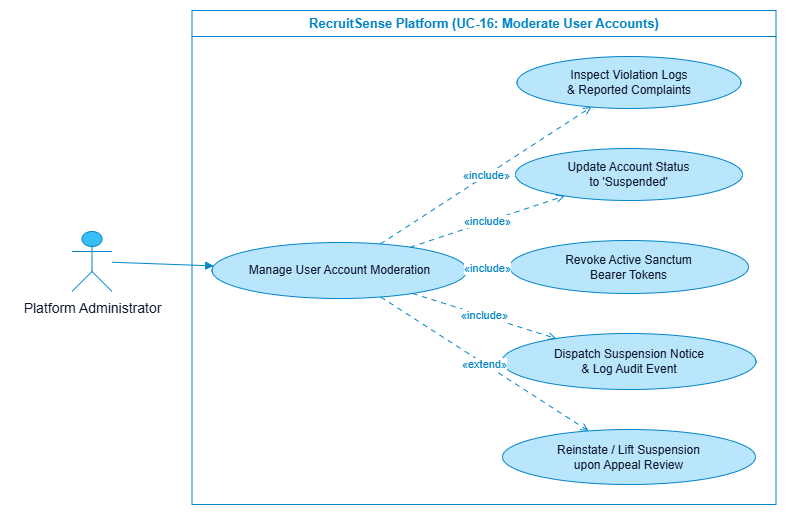
\includegraphics[width=0.65\linewidth]{figures/usecase_moderate_users.png}
\caption{Moderate User Accounts and Suspensions Use Case Diagram}
\label{fig:uc16_diag}
\end{figure}

\begin{table}[H]
\centering
\small
\caption{Use Case: Moderate User Accounts and Suspensions (UC-16)}
\label{tab:uc16_spec}
\begin{tabular}{|p{3.2cm}|p{5.5cm}|p{5.5cm}|}
\hline
\textbf{Use Case ID:} & \multicolumn{2}{p{11.4cm}|}{UC-16} \\ \hline
\textbf{Use Case Name:} & \multicolumn{2}{p{11.4cm}|}{Moderate User Accounts and Suspensions} \\ \hline
\textbf{Created By:} & \multicolumn{2}{p{11.4cm}|}{Hamza Zahoor} \\ \hline
\textbf{Last Updated By:} & \multicolumn{2}{p{11.4cm}|}{Haseeb Ahmed} \\ \hline
\textbf{Actors:} & \multicolumn{2}{p{11.4cm}|}{Platform Administrator} \\ \hline
\textbf{Description:} & \multicolumn{2}{p{11.4cm}|}{Admin reviews reported user behavior and applies suspensions or restrictions.} \\ \hline
\textbf{Trigger:} & \multicolumn{2}{p{11.4cm}|}{Admin accesses user moderation panel.} \\ \hline
\textbf{Preconditions:} & \multicolumn{2}{p{11.4cm}|}{Admin is authenticated; reported user exists.} \\ \hline
\textbf{Post conditions:} & \multicolumn{2}{p{11.4cm}|}{User status changed to \texttt{'suspended'}; active sessions terminated.} \\ \hline
\multirow{4}{*}{\textbf{Normal Flow:}} & \multicolumn{1}{c|}{\textbf{Actor}} & \multicolumn{1}{c|}{\textbf{System}} \\ \cline{2-3}
& 1. Admin selects flagged user account. & 2. System loads profile history and recent activity logs. \vspace{2pt} \\
& 3. Admin reviews violation logs and submitted reports. & 4. System displays action options and suspension duration controls. \vspace{2pt} \\
& 5. Admin confirms suspension and enters reason. & 6. System sets \texttt{users.status = 'suspended'}, revokes Sanctum tokens, and sends email notice. \\ \hline
\textbf{Alternative Flows:} & \multicolumn{2}{p{11.4cm}|}{1. Admin lifts previous suspension after appeal review.} \\ \hline
\textbf{Exceptions:} & \multicolumn{2}{p{11.4cm}|}{1. Admin attempts to suspend own account (Action blocked).} \\ \hline
\end{tabular}
\end{table}

\subsection{View System Analytics and Audit Logs (UC-17)}
Administrators can inspect global recruitment analytics, including total registered candidates, verified employers, active job listings, total resumes parsed, average ATS match scores across categories, and system API logs. This workflow is depicted in Figure \ref{fig:uc17_diag} and summarised in Table \ref{tab:uc17_spec}.

\begin{figure}[H]
\centering
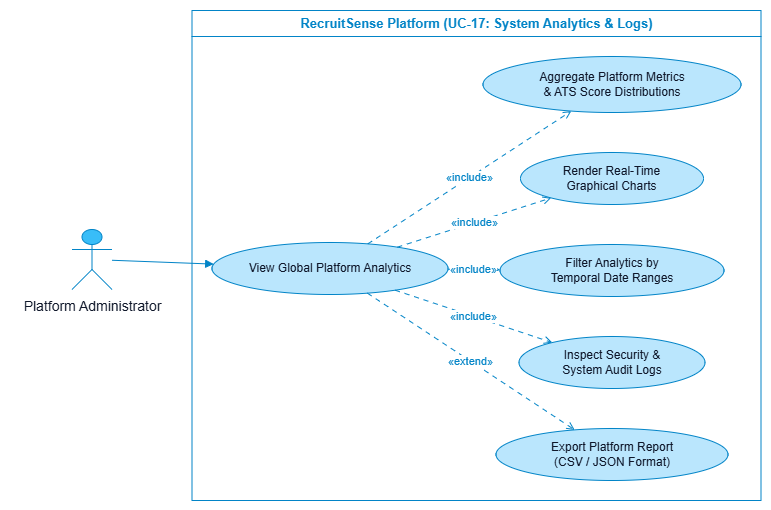
\includegraphics[width=0.65\linewidth]{figures/usecase_analytics.png}
\caption{View System Analytics and Audit Logs Use Case Diagram}
\label{fig:uc17_diag}
\end{figure}

\begin{table}[H]
\centering
\small
\caption{Use Case: View System Analytics and Audit Logs (UC-17)}
\label{tab:uc17_spec}
\begin{tabular}{|p{3.2cm}|p{5.5cm}|p{5.5cm}|}
\hline
\textbf{Use Case ID:} & \multicolumn{2}{p{11.4cm}|}{UC-17} \\ \hline
\textbf{Use Case Name:} & \multicolumn{2}{p{11.4cm}|}{View System Analytics and Audit Logs} \\ \hline
\textbf{Created By:} & \multicolumn{2}{p{11.4cm}|}{Hamza Zahoor} \\ \hline
\textbf{Last Updated By:} & \multicolumn{2}{p{11.4cm}|}{Haseeb Ahmed} \\ \hline
\textbf{Actors:} & \multicolumn{2}{p{11.4cm}|}{Platform Administrator} \\ \hline
\textbf{Description:} & \multicolumn{2}{p{11.4cm}|}{Administrator monitors global platform statistics, ATS screening metrics, and activity logs.} \\ \hline
\textbf{Trigger:} & \multicolumn{2}{p{11.4cm}|}{Admin opens Admin Analytics Dashboard.} \\ \hline
\textbf{Preconditions:} & \multicolumn{2}{p{11.4cm}|}{Admin is authenticated with root permissions.} \\ \hline
\textbf{Post conditions:} & \multicolumn{2}{p{11.4cm}|}{Statistical visual metrics and system audit logs rendered.} \\ \hline
\multirow{4}{*}{\textbf{Normal Flow:}} & \multicolumn{1}{c|}{\textbf{Actor}} & \multicolumn{1}{c|}{\textbf{System}} \\ \cline{2-3}
& 1. Admin navigates to Analytics tab. & 2. System aggregates database metrics (users, jobs, applications, average ATS scores). \vspace{2pt} \\
& 3. Admin selects date range filter. & 4. System updates graphical charts and performance summaries in real time. \vspace{2pt} \\
& 5. Admin inspects audit log table. & 6. System renders chronological security audit logs. \\ \hline
\textbf{Alternative Flows:} & \multicolumn{2}{p{11.4cm}|}{1. Admin exports platform health metrics to CSV/JSON report.} \\ \hline
\textbf{Exceptions:} & \multicolumn{2}{p{11.4cm}|}{1. Database query timeout during high-volume aggregation.} \\ \hline
\end{tabular}
\end{table}

\subsection{Update Profile and Professional Summary (UC-18)}
Job seekers and recruiters can update their personal profiles, headline, biography, portfolio links, location, and technical skill tags. The system validates input fields, updates the database, and refreshes the user's profile state. This workflow is depicted in Figure \ref{fig:uc18_diag} and summarised in Table \ref{tab:uc18_spec}.

\begin{figure}[H]
\centering
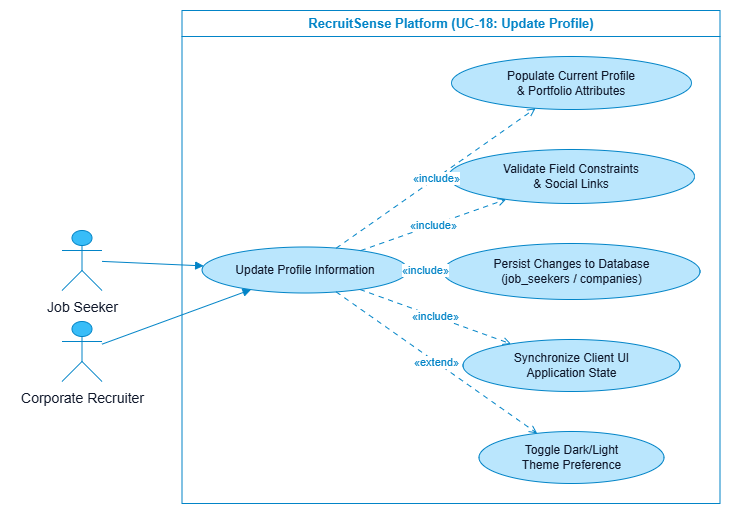
\includegraphics[width=0.65\linewidth]{figures/usecase_profile.png}
\caption{Update Profile and Professional Summary Use Case Diagram}
\label{fig:uc18_diag}
\end{figure}

\begin{table}[H]
\centering
\small
\caption{Use Case: Update Profile and Professional Summary (UC-18)}
\label{tab:uc18_spec}
\begin{tabular}{|p{3.2cm}|p{5.5cm}|p{5.5cm}|}
\hline
\textbf{Use Case ID:} & \multicolumn{2}{p{11.4cm}|}{UC-18} \\ \hline
\textbf{Use Case Name:} & \multicolumn{2}{p{11.4cm}|}{Update Profile and Professional Summary} \\ \hline
\textbf{Created By:} & \multicolumn{2}{p{11.4cm}|}{Hamza Zahoor} \\ \hline
\textbf{Last Updated By:} & \multicolumn{2}{p{11.4cm}|}{Haseeb Ahmed} \\ \hline
\textbf{Actors:} & \multicolumn{2}{p{11.4cm}|}{Registered User (Job Seeker, Recruiter)} \\ \hline
\textbf{Description:} & \multicolumn{2}{p{11.4cm}|}{Modify personal details, bio, skill tags, contact details, and account preferences.} \\ \hline
\textbf{Trigger:} & \multicolumn{2}{p{11.4cm}|}{User clicks ``Edit Profile'' on their profile dashboard.} \\ \hline
\textbf{Preconditions:} & \multicolumn{2}{p{11.4cm}|}{User is authenticated.} \\ \hline
\textbf{Post conditions:} & \multicolumn{2}{p{11.4cm}|}{Profile record updated in database; updated data reflected in client state.} \\ \hline
\multirow{4}{*}{\textbf{Normal Flow:}} & \multicolumn{1}{c|}{\textbf{Actor}} & \multicolumn{1}{c|}{\textbf{System}} \\ \cline{2-3}
& 1. User accesses profile settings. & 2. System loads current profile data from database. \vspace{2pt} \\
& 3. User edits bio, location, headline, or adds new skills. & 4. System validates character lengths and inputs. \vspace{2pt} \\
& 5. User clicks ``Save Profile''. & 6. System updates \texttt{job\_seekers} or \texttt{companies} table and displays success alert. \\ \hline
\textbf{Alternative Flows:} & \multicolumn{2}{p{11.4cm}|}{1. User toggles Dark/Light theme mode in profile settings.} \\ \hline
\textbf{Exceptions:} & \multicolumn{2}{p{11.4cm}|}{1. Invalid input format (System highlights erroneous fields).} \\ \hline
\end{tabular}
\end{table}

\subsection{Report Suspicious or Fraudulent Job Posting (UC-19)}
Job seekers can report misleading, discriminatory, or fraudulent job listings directly through the job details interface. The report includes category selection (e.g., Fake Listing, Scam, Inappropriate Content) and supporting remarks, adding the case to the admin moderation queue. This workflow is depicted in Figure \ref{fig:uc19_diag} and summarised in Table \ref{tab:uc19_spec}.

\begin{figure}[H]
\centering
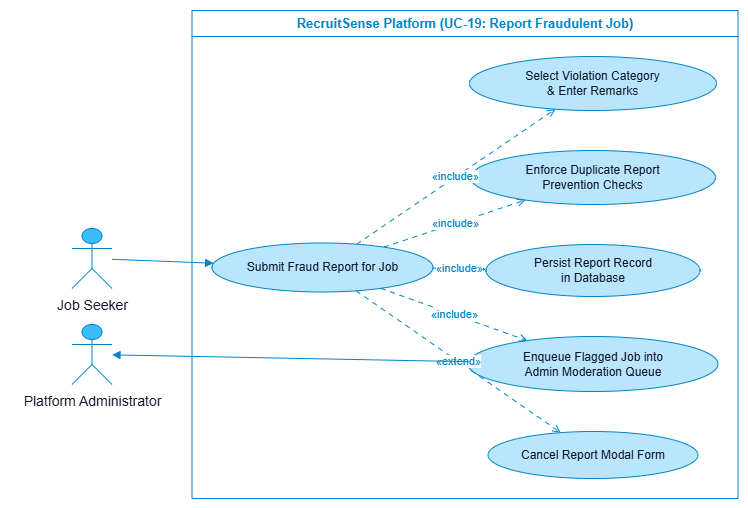
\includegraphics[width=0.65\linewidth]{figures/usecase_report_job.png}
\caption{Report Suspicious or Fraudulent Job Posting Use Case Diagram}
\label{fig:uc19_diag}
\end{figure}

\begin{table}[H]
\centering
\small
\caption{Use Case: Report Suspicious or Fraudulent Job Posting (UC-19)}
\label{tab:uc19_spec}
\begin{tabular}{|p{3.2cm}|p{5.5cm}|p{5.5cm}|}
\hline
\textbf{Use Case ID:} & \multicolumn{2}{p{11.4cm}|}{UC-19} \\ \hline
\textbf{Use Case Name:} & \multicolumn{2}{p{11.4cm}|}{Report Suspicious or Fraudulent Job Posting} \\ \hline
\textbf{Created By:} & \multicolumn{2}{p{11.4cm}|}{Hamza Zahoor} \\ \hline
\textbf{Last Updated By:} & \multicolumn{2}{p{11.4cm}|}{Haseeb Ahmed} \\ \hline
\textbf{Actors:} & \multicolumn{2}{p{11.4cm}|}{Job Seeker} \\ \hline
\textbf{Description:} & \multicolumn{2}{p{11.4cm}|}{Candidate flags a job posting for policy violations or fraudulent behavior.} \\ \hline
\textbf{Trigger:} & \multicolumn{2}{p{11.4cm}|}{Candidate clicks ``Report Job'' on a job vacancy modal.} \\ \hline
\textbf{Preconditions:} & \multicolumn{2}{p{11.4cm}|}{Candidate is authenticated; job posting is active.} \\ \hline
\textbf{Post conditions:} & \multicolumn{2}{p{11.4cm}|}{Report record inserted into database; listing flagged for admin review.} \\ \hline
\multirow{4}{*}{\textbf{Normal Flow:}} & \multicolumn{1}{c|}{\textbf{Actor}} & \multicolumn{1}{c|}{\textbf{System}} \\ \cline{2-3}
& 1. Candidate clicks ``Report Job''. & 2. System displays report modal with category options. \vspace{2pt} \\
& 3. Candidate selects violation category and inputs explanation. & 4. System validates completeness of explanation. \vspace{2pt} \\
& 5. Candidate clicks ``Submit Report''. & 6. System persists report, notifies admin queue, and confirms submission to user. \\ \hline
\textbf{Alternative Flows:} & \multicolumn{2}{p{11.4cm}|}{1. Candidate cancels report modal before submitting.} \\ \hline
\textbf{Exceptions:} & \multicolumn{2}{p{11.4cm}|}{1. Candidate has already submitted a report for this job.} \\ \hline
\end{tabular}
\end{table}

\subsection{Review Reported Content and Job Postings (UC-20)}
Administrators review reported job postings and candidate complaints, examine evidence, and take administrative action---such as removing the listing, warning the employer, or dismissing false reports. This workflow is depicted in Figure \ref{fig:uc20_diag} and summarised in Table \ref{tab:uc20_spec}.

\begin{figure}[H]
\centering
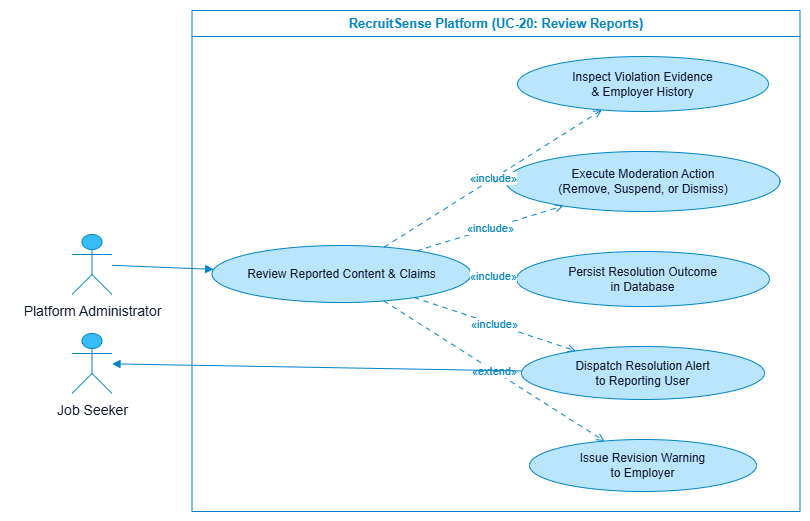
\includegraphics[width=0.65\linewidth]{figures/usecase_review_reports.png}
\caption{Review Reported Content and Job Postings Use Case Diagram}
\label{fig:uc20_diag}
\end{figure}

\begin{table}[H]
\centering
\small
\caption{Use Case: Review Reported Content and Job Postings (UC-20)}
\label{tab:uc20_spec}
\begin{tabular}{|p{3.2cm}|p{5.5cm}|p{5.5cm}|}
\hline
\textbf{Use Case ID:} & \multicolumn{2}{p{11.4cm}|}{UC-20} \\ \hline
\textbf{Use Case Name:} & \multicolumn{2}{p{11.4cm}|}{Review Reported Content and Job Postings} \\ \hline
\textbf{Created By:} & \multicolumn{2}{p{11.4cm}|}{Hamza Zahoor} \\ \hline
\textbf{Last Updated By:} & \multicolumn{2}{p{11.4cm}|}{Haseeb Ahmed} \\ \hline
\textbf{Actors:} & \multicolumn{2}{p{11.4cm}|}{Platform Administrator} \\ \hline
\textbf{Description:} & \multicolumn{2}{p{11.4cm}|}{Administrator mediates complaints, reviews flagged content, and applies policy enforcement.} \\ \hline
\textbf{Trigger:} & \multicolumn{2}{p{11.4cm}|}{Administrator accesses the Admin Reports Queue.} \\ \hline
\textbf{Preconditions:} & \multicolumn{2}{p{11.4cm}|}{Administrator is authenticated with moderation privileges.} \\ \hline
\textbf{Post conditions:} & \multicolumn{2}{p{11.4cm}|}{Reported issue is resolved; listing removed or report dismissed.} \\ \hline
\multirow{4}{*}{\textbf{Normal Flow:}} & \multicolumn{1}{c|}{\textbf{Actor}} & \multicolumn{1}{c|}{\textbf{System}} \\ \cline{2-3}
& 1. Admin opens reported content queue. & 2. System displays list of unresolved reports. \vspace{2pt} \\
& 3. Admin selects report to inspect. & 4. System presents job details, employer history, and reporter comments. \vspace{2pt} \\
& 5. Admin decides outcome (Remove Listing, Suspend Employer, or Dismiss). & 6. System executes decision, updates database, and notifies reporting user. \\ \hline
\textbf{Alternative Flows:} & \multicolumn{2}{p{11.4cm}|}{1. Admin sends warning message to employer requesting listing revision.} \\ \hline
\textbf{Exceptions:} & \multicolumn{2}{p{11.4cm}|}{1. Job posting was already deleted by owner prior to review.} \\ \hline
\end{tabular}
\end{table}

\section{Chapter Summary}
This chapter comprehensively documented the requirement specifications for \textbf{RecruitSense}. It analyzed the operational bottlenecks of existing manual and keyword-based recruitment systems, articulated the proposed platform capabilities, established the functional requirements (FR-01 to FR-20) and non-functional quality constraints (NFR-01 to NFR-10), presented the overall system use case model, and provided formal tabular specifications alongside native vector diagrams for 20 distinct use cases. These specifications establish a rigorous foundation for the architectural and system design detailed in Chapter \ref{chap:design}.
